\documentclass[12pt]{article}
\usepackage[margin=1in]{geometry}
\usepackage{microtype}
\usepackage{xurl}
\usepackage[table]{xcolor}
\usepackage{hyperref}
\usepackage{graphicx}
\hypersetup{
  colorlinks=true,
  urlcolor=blue,
  linkcolor=blue,
  citecolor=blue
}
\setlength{\parindent}{0pt}
\setlength{\parskip}{0.8em}
\setlength{\emergencystretch}{4em}
\sloppy

\begin{document}
\begin{center}
{\LARGE San Jose State University}\\[0.5em]
{\LARGE CS 147 - Computer Architecture}\\[0.5em]
{\LARGE Class Project - Phase 2}
\end{center}

\vspace{2em}

\subsection*{Overall Timeline and Grade Distribution}
\begin{center}
\begin{tabular}{|l|l|l|}
\hline
\textbf{Due Date} & \multicolumn{2}{l|}{\textbf{Project Component}} \\
\hline
2/26/26 & Design Review & (5\% of project grade) \\
\hline
3/10/26 & Phase \#1 & (15\% of project grade) \\
\hline
\rowcolor{black!8}
4/7/26 & Phase \#2 & (30\% of project grade) \\
\hline
\rowcolor{black!8}
4/16/26 & Phase \#2.1 & (10\% of project grade) \\
\hline
\rowcolor{black!8}
N/A & Phase \#2.2 & (Optional) \\
\hline
\rowcolor{black!8}
4/23/26 & Phase \#2.3 Caching & (10\% of project grade) \\
\hline
5/7/26 & Phase \#3 & (30\% of project grade) \\
\hline
\end{tabular}
\end{center}

\section*{Phase \#2 --- Pipelined Design with Perfect Memory (30\% of project grade)}

At this point, the pipelined version of your design needs to be running correctly, but no optimizations are needed yet.
Correctly means that it must detect and do the right thing on pipeline hazards (e.g., stall).
You will still use the single-cycle memory model.
We will follow similar protocol as demo1.
We will run your tests and ask students with any failures to sign up for a demo with us.

\subsection*{Required student\_custom tests}
You must write at least two additional custom tests for pipelining and include them in the student custom test flow.
Specifically, place at least two test programs in:
\begin{quote}
\texttt{./assignments/project/testprograms/student\_custom/}
\end{quote}
and add them to:
\begin{quote}
\texttt{./assignments/project/testprograms/student\_custom/all\_phase\_2.list}
\end{quote}

Writing more tests is strongly encouraged and will simplify debugging.
At minimum, the presence of at least two student custom tests is required.
The presence of a minimum of two (passing) student custom tests will be factored into the Phase 2 grade.

\subsection*{Instruction timeline}
You must create and submit a document which should explain the behavior of your processor for the \texttt{perf-test-dep-ldst.asm} test.
Please use the following format:

\begin{center}
\begin{tabular}{|l|l|l|}
\hline
\textbf{Cycle} & \textbf{Instruction Retired} & \textbf{Reason} \\
\hline
1 & & \\
\noalign{{\color{black!35}\hrule height 0.25pt}}
2 & & \\
\noalign{{\color{black!35}\hrule height 0.25pt}}
\vdots & \vdots & \vdots \\
\noalign{{\color{black!35}\hrule height 0.25pt}}
Etc. & & \\
\hline
\end{tabular}
\end{center}

The instruction retired (we will discuss what retired means in class, but essentially for our 5-stage in-order processor it means what is in Write Back that cycle) would either be one of the instructions from the test program or a ``NOP'' if dependencies necessitate any stall cycles.
The reason column would explain why a stall was needed in that instance.

Please include this information in a PDF file titled \texttt{instruction\_timeline.pdf}, located at:
\begin{quote}
\texttt{./demo2/writeup/instruction\_timeline.pdf}
\end{quote}

\subsection*{Synthesis}
You should also synthesize your processor and submit the results of synthesis, including the area, cell, and timing reports.  This is similar to what you did for Lab 3.

\subsection*{Submitting}
To generate your Phase 2 submission file, use:
\begin{quote}
\texttt{./run build\_submission project phase\_2}
\end{quote}

This follows the same submission workflow used in Phase 1: run the Phase 2 test flow, package the expected files, and produce a submission zip for upload.

Your generated submission zip will be written to:
\begin{quote}
\path{./generated_turnins/project_phase_2}
\end{quote}

Upload the generated zip file to the corresponding Phase 2 Gradescope assignment.

\subsection*{Testing Commands}
Base command form:
\begin{quote}
\texttt{./run test [-v] project phase\_2 [subtest]}
\end{quote}

Subphase command form:
\begin{quote}
\texttt{./run test [-v] project phase\_2\_x [subtest]}
\end{quote}
\texttt{x} is the follow-on phase to be tested. Running \texttt{phase\_2\_1} or \texttt{phase\_2\_2} already selects only that subphase.

Cache-selection form for Phase 2.3:
\begin{quote}
\texttt{./run test [-v] project phase\_2\_3 [-direct|-associative] [-only] [subtest]}
\end{quote}
By default, \texttt{phase\_2\_3} runs both cache implementations. The \texttt{-only} flag is used only with \texttt{phase\_2\_3} cache selection, together with \texttt{-direct} or \texttt{-associative}, to run just that selected cache implementation.

\subsection*{Required Test Categories}
The base \texttt{phase\_2} grading pass evaluates:
\begin{enumerate}
  \item Your student custom tests (\texttt{student\_custom})
  \item Simple instruction tests (\texttt{inst\_tests})
  \item Complex tests from demo1 (\texttt{complex\_demo1})
  \item Random tests for demo1:
    \begin{enumerate}
      \item \texttt{rand\_simple}
      \item \texttt{rand\_complex}
      \item \texttt{rand\_ctrl}
      \item \texttt{rand\_mem}
    \end{enumerate}
  \item Random/complex tests for demo2 (\texttt{complex\_demo2})
\end{enumerate}

\textbf{Additional categories are included when you run \texttt{phase\_2\_x} commands, as described in the Testing Commands section above.}

The initial Phase 2 grading pass is based on \texttt{phase\_2} categories. The 2.1/2.2/2.3 Follow-on phases are exercised by their corresponding \texttt{phase\_2\_x} commands.

A brief note of caution: if your \texttt{all\_phase\_2.list} has $>$ 100 failures, the test runner will stop running tests from that list --- please make sure to check your logs if you have many failures.

Running all tests can take significant time. Plan ahead and avoid waiting until the deadline window.

\subsection*{Follow-on phases}
The next phases are intended as incremental extensions to your Phase 2 pipeline implementation.
Phase \#2.1 and the Cache Demo (\#2.3) are required project milestones.
Phase \#2.2 is optional.
Make sure your design passes the expected tests at each stage.

\section*{Phase \#2.1 --- Pipelined Design with Aligned Memory (10\% of project grade)}
\textbf{This milestone is required.}

At this step, replace the original single-cycle memory with the Aligned single-cycle memory.
This is a very similar module, but it has an \texttt{err} output that is generated on unaligned memory accesses.
Your processor should halt when an error occurs.
Verify your design.

If you want to test, you can test with the \texttt{unaligned.list} test set:

\begin{quote}
\texttt{./run test project phase\_2\_1}
\end{quote}
This runs the Phase 2.1 category.

\subsection*{Aligned single-cycle memory specification (summary)}
Before building your cache, you should use this memory to update and test your processor's interface to properly handle unaligned accesses.
Many processors (e.g., MIPS) are byte addressable, but require that all accesses be aligned to their natural size (i.e., byte loads and stores can access any individual byte, but word loads and stores must access aligned words).

Since your processor only has word loads and stores, this is pretty simple.
(To support byte stores, the memory would need byte write enable signals; to support byte loads, either the memory or the processor needs a mux to select the right byte.)

Notice that the memory always returns aligned data even on a misaligned load, and memory does not store anything on a misaligned store.

The Verilog source is provided at:
\begin{quote}
\texttt{./demo2/verilog/phase2\_1/memory2c\_align.v}
\end{quote}

Since your single-cycle design must fetch instructions as well as read or write data in the same cycle, you will want to use two instances of this memory --- one for data, and one for instructions.

\begin{center}
\begin{figure}[h]
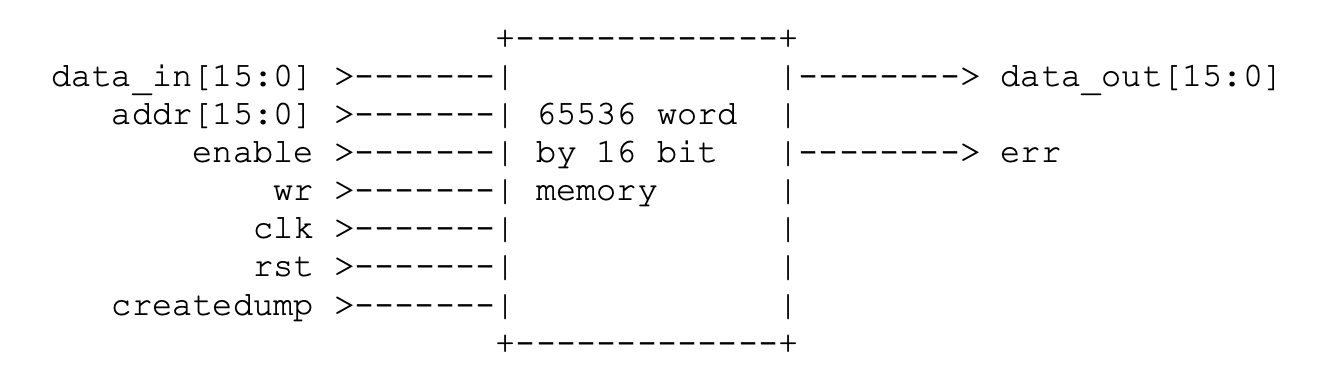
\includegraphics[width=\textwidth]{src/memory-info.png}
\end{figure}
\end{center}

During each cycle, the ``enable" and ``wr" inputs determine what function the memory
will perform. On an unaligned access err is set.

\begin{center}
\begin{tabular}{|l|l|l|l|l|} \hline
enable & wr & Function & data\_out & err \\ \hline
0 & X & No operation & 0 & 0 \\ \hline
1 &.0 & Read & M[addr] & 0 \\ \hline
1 & 1 & Write & Write data\_in & 0 \\ \hline
1 & X & X & if (addr[0]) set & 1 \\ \hline
\end{tabular}
\end{center}

\section*{Phase \#2.2 --- Pipelined Design with Stalling Memory (Optional)}
\textbf{No submission required. This is optional.}

At this step, replace the single-cycle memory with the Stalling memory.
This is a very similar module, but has \texttt{stall} and \texttt{done} signals similar to the cache you will build.
Your pipeline will need to stall to handle these conditions.
Verify your design.

\begin{itemize}
  \item \textbf{Instruction memory:} First replace your instruction memory module with this stalling memory; keep your data memory module the same (i.e., aligned perfect memory from previous step).
  Verify your design.
  This will be easier to debug, as only one module's behavior has changed.
  \item \textbf{Data memory:} Now, replace your data memory module alone with this stalling memory; revert your instruction memory module back to the aligned perfect memory.
  Verify your design.
  This will be easier to debug, as only one module's behavior has changed.
  \item \textbf{Instruction and Data memory:} Now change both instruction and data memories to the stalling memory design.
  Verify your design.
\end{itemize}

\subsection*{Stalling memory specification (seed control)}
This module has an interface identical to the cache interface in \texttt{mem\_system\_hier.v}.

Examining the source file \texttt{./demo2/verilog/phase2\_2/stallmem.v}, you will see \texttt{rand\_pat}, a shift register which controls the \texttt{ready} output.
This is a random 32-bit number.
You can change its value by changing the seed used for random number generation.

To run the stalling-memory category:
\begin{quote}
\texttt{./run test project phase\_2\_2}
\end{quote}
For seed-specific debugging, use interactive simulation and/or adjust the seed initialization in \texttt{./demo2/verilog/phase2\_2/stallmem.v}.

\section*{Phase \#2.3 --- Cache Demo: Working Cache Memory System (10\% of project grade)}

In this phase you will implement a cache-based memory system to replace the idealized memory used earlier in the project.
Your final processor will use both an instruction cache and a data cache. For this stage of the project you will design and
verify the cache subsystem that will ultimately be integrated into your processor design.

You will first implement and test a \textbf{direct-mapped cache}. After that design is working and verified, you will extend
it to a \textbf{two-way set associative cache}.

The cache storage arrays and the main memory module are already provided. Your task is to implement the
\textbf{memory system controller} that coordinates the cache and memory modules.

\subsection*{Project Files}

The cache files for this stage are organized under:
\begin{quote}
\texttt{./demo2/verilog/phase2\_3/}
\end{quote}
Each cache implementation directory contains a number of modules.

\begin{center}
\begin{tabular}{|l|p{10cm}|}
\hline
\textbf{File} & \textbf{Description} \\
\hline
cache.v & Cache storage structures (data, tag, valid, dirty) \\
clkrst.v & Clock and reset module \\
final\_memory.v & Memory bank implementation \\
four\_bank\_mem.v & Four-banked memory wrapper \\
mem.addr & Example address trace file \\
memc.v & Data storage module used by cache \\
memv.v & Valid-bit storage module used by cache \\
mem\_system\_hier.v & Top-level wrapper used for testing \\
mem\_system\_perfbench.v & Trace-based testbench \\
mem\_system\_randbench.v & Random testbench \\
mem\_system\_ref.v & Reference implementation used by testbench \\
mem\_system.v & Memory system module \textbf{(this is the file you modify)} \\
*.syn.v & Synthesizable memory modules \\
\hline
\end{tabular}
\end{center}

In most cases, \texttt{mem\_system.v} is the only module that must be modified.

\subsection*{Four-Banked Memory}

The provided memory module models a modern memory system by dividing memory into four independent banks.

\begin{itemize}
\item Memory is \textbf{64 KB}
\item Word size is \textbf{16 bits}
\item Memory is \textbf{byte addressable but word aligned}
\item Memory is split into \textbf{four banks}
\end{itemize}

\begin{figure}
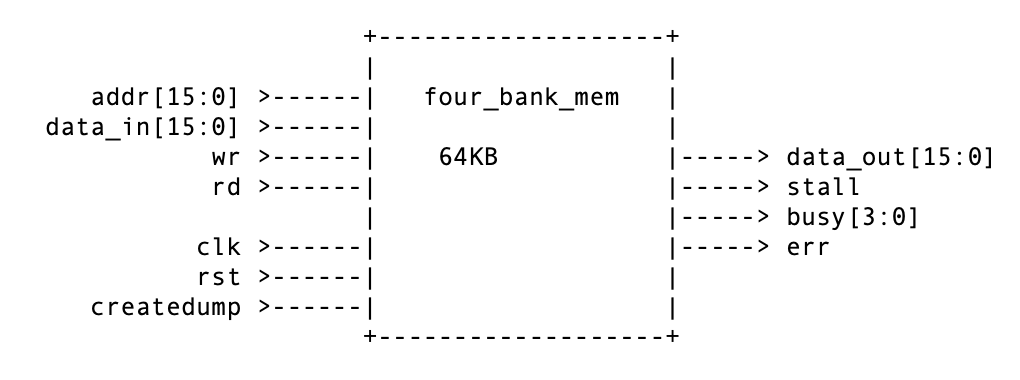
\includegraphics{src/four_bank_mem.png}
\caption{Four Bank Memory}
\label{fig1}
\end{figure}

The least significant address bits determine the memory bank. Because addresses are word aligned, bit 0 is always zero.
Therefore bits \texttt{Addr[2:1]} determine the bank.

If two accesses target the same bank within four cycles, the second request will stall.

Figure~\ref{fig1} shows the external interface to the module.  Figure~\ref{fig2:Timing} shows the timing specification.

Each signal is described below:

\begin{center}
\begin{tabular}{|l|c|c|p{8cm}|}
\hline
Signal & Direction & Width & Description \\
\hline
Addr & In & 16 & Address of the memory operation \\
DataIn & In & 16 & Data written during write operations \\
wr & In & 1 & Write enable signal \\
rd & In & 1 & Read enable signal \\
clk & In & 1 & Clock \\
rst & In & 1 & Reset \\
createdump & In & 1 & Dump memory contents to files \\
DataOut & Out & 16 & Data returned on reads \\
stall & Out & 1 & Indicates bank conflict \\
Busy & Out & 4 & Busy status for each bank \\
err & Out & 1 & Raised on unaligned accesses \\
\hline
\end{tabular}
\end{center}


\begin{figure}
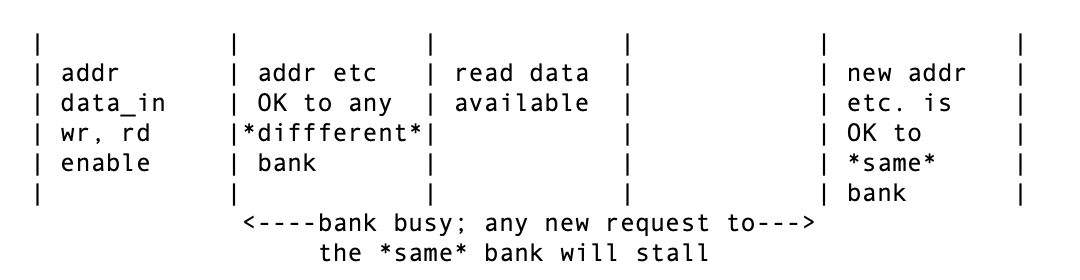
\includegraphics[width=\textwidth]{src/timing.png}
\caption{Timing}
\label{fig2:Timing}
\end{figure}

\subsection*{Cache Organization}

\begin{figure}
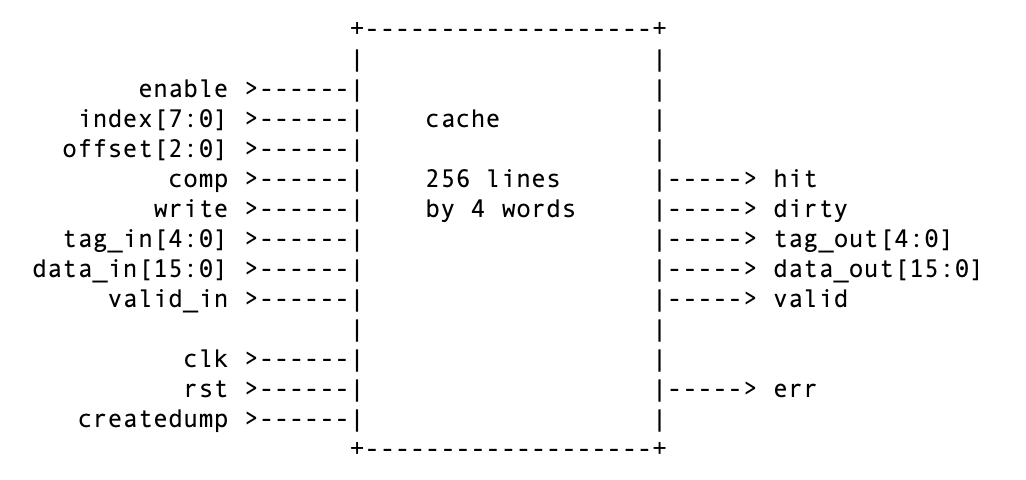
\includegraphics{src/cache.png}
\caption{External Cache Interface}
\label{fig3:cache}
\end{figure}

The cache contains \textbf{256 lines}. Each line contains the following fields (see Figure~\ref{fig4:cache-org}):
\begin{itemize}
\item Valid bit
\item Dirty bit
\item 5-bit tag
\item Four 16-bit words
\end{itemize}

\begin{figure}
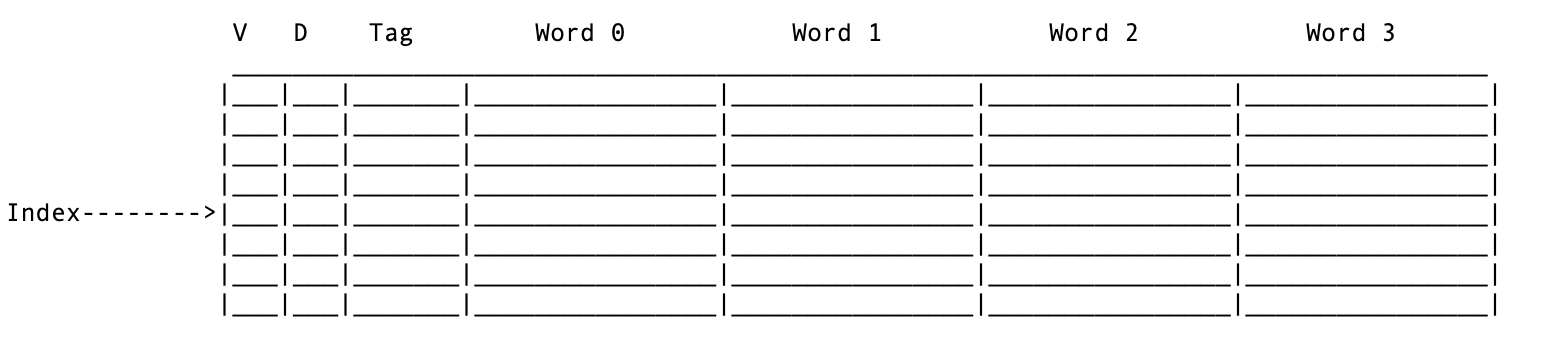
\includegraphics[width=\textwidth]{src/cache_org.png}
\caption{Cache Organization}
\label{fig4:cache-org}
\end{figure}


Figure~\ref{fig3:cache} shows the external cache interface.  Each interface signal is described in table below (see Table~\ref{tab:cache-signals}):

\begin{center}
\begin{table}
\begin{tabular}{|l|c|c|p{8cm}|}
\hline
Signal & Direction & Width & Description \\
\hline
enable & In & 1 & Enables cache access \\
index & In & 8 & Cache index \\
offset & In & 3 & Selects word within cache line \\
comp & In & 1 & Enables tag comparison \\
write & In & 1 & Write enable \\
tag\_in & In & 5 & Tag value from processor \\
data\_in & In & 16 & Data written to cache \\
valid\_in & In & 1 & Valid bit written during fills \\
clk & In & 1 & Clock \\
rst & In & 1 & Reset \\
createdump & In & 1 & Dump cache contents \\
\hline
hit & Out & 1 & Tag match indicator \\
dirty & Out & 1 & Dirty bit state \\
tag\_out & Out & 5 & Tag read during eviction \\
data\_out & Out & 16 & Data read from cache \\
valid & Out & 1 & Valid bit state \\
err & Out & 1 & Error condition \\
\hline
\end{tabular}
\caption{Cache Interface Signals}
\label{tab:cache-signals}
\end{table}
\end{center}

\subsection*{Cache Access Modes}

The cache operates using two control signals: \texttt{comp} and \texttt{write}. The four possible combinations are:

\textbf{Compare Read (comp=1, write=0)}

Used during load instructions.

\begin{itemize}
\item Tag is compared with stored tag
\item If hit, data is returned immediately
\item If miss, the valid and dirty bits of the current line are observed
\end{itemize}

\textbf{Compare Write (comp=1, write=1)}

Used during store instructions.

\begin{itemize}
\item If hit, data is written to the cache line
\item Dirty bit is set
\item If miss, cache contents are not modified
\end{itemize}

\textbf{Access Read (comp=0, write=0)}

Used internally when evicting a cache line.

\begin{itemize}
\item Tag, valid, dirty, and data values are read from the cache
\end{itemize}

\textbf{Access Write (comp=0, write=1)}

Used when filling a cache line from memory.

\begin{itemize}
\item Data and tag are written into the cache
\item Valid bit is set
\item Dirty bit is cleared
\end{itemize}

\subsection*{State Machine}

You must design a state machine to control cache behavior. Either a Mealy or Moore machine may be used
(though Moore designs are typically easier).

Your controller must manage:

\begin{itemize}
\item Cache hit detection
\item Cache misses
\item Memory read operations
\item Dirty-line writebacks
\item Cache line fills
\item Stall and done signaling
\end{itemize}

\textbf{A state diagram for your cache controller must be submitted as part of this phase.}

\subsection*{Direct-Mapped Cache}

First implement a direct-mapped cache in the directory:

\begin{quote}
\texttt{./demo2/verilog/phase2\_3/cache\_direct/}
\end{quote}

You should thoroughly test this version before proceeding to the associative version.

\subsection*{Synthesis}
You will need to run synthesis on your direct mapped cache and verify that it does not produce any errors. You should turn in all of the reports generated by synthesis.

Your synthesis results should be placed in this directory: 
\begin{quote}
\texttt{./demo2/verilog/phase2\_3/cache\_direct/}
\end{quote}

\subsection*{Testing}

Use the project test wrapper for this follow-on phase:
\begin{quote}
\texttt{./run test project phase\_2\_3}
\end{quote}
By default, this runs \textbf{both} cache implementations (direct-mapped and two-way associative).

To run only one cache implementation within Phase 2.3, use:
\begin{quote}
\texttt{./run test project phase\_2\_3 -direct -only}
\end{quote}
\begin{quote}
\texttt{./run test project phase\_2\_3 -associative -only}
\end{quote}

Verbose mode / targeted debugging:
\begin{quote}
\texttt{./run test -v project phase\_2\_3 [subtest]}
\end{quote}

\subsection*{Two-Way Set-Associative Cache}

After verifying the direct-mapped cache, extend your design to a two-way set associative cache
in directory:

\begin{quote}
\texttt{./demo2/verilog/phase2\_3/cache\_assoc/}
\end{quote}

Two cache modules are instantiated, and hit detection is performed across both ways.

\subsection*{Replacement Policy}

To ensure deterministic grading, you must implement the following pseudo-random replacement policy.

\begin{enumerate}
\item Maintain a flip-flop named \texttt{victimway}.
\item Initialize \texttt{victimway} to zero.
\item On each cache read or write, invert \texttt{victimway}.
\item If both cache ways are valid during replacement, select the way indicated by \texttt{victimway}.
\item If one way in the indexed set is invalid, place the new block in that invalid way instead of evicting a valid block. Don't evict unless the set is full.
\end{enumerate}

\subsection*{Synthesis}
You will also need to synthesize your set-associative cache. You should turn in all of the reports generated by synthesis.
Your synthesis results should be placed in the directory:
\begin{quote}
\texttt{./demo2/verilog/phase2\_3/cache\_assoc/}
\end{quote}

\subsection*{Submission}

Use the standard submission wrapper:
\begin{quote}
\texttt{./run build\_submission project phase\_2}
\end{quote}

The generated submission zip is written to:
\begin{quote}
\texttt{./generated\_turnins/project\_phase\_2/}
\end{quote}

Your Phase 2.3 work must be present in:
\begin{quote}
\texttt{./demo2/verilog/phase2\_3/cache\_direct/}

\texttt{./demo2/verilog/phase2\_3/cache\_assoc/}
\end{quote}

Required artifacts include:

\begin{itemize}
\item Your cache controller state diagram (\texttt{state\_machine.pdf})
\item All Verilog modules
\item Any additional files required by your Phase 2.3 implementation/testing flow
\end{itemize}

Place \texttt{state\_machine.pdf} in:
\begin{quote}
\texttt{./demo2/writeup/state\_machine.pdf}
\end{quote}

\end{document}
